% !TeX root=../main.tex
\chapter{معادلات دیفرانسیل و آنالیز عددی}
%\thispagestyle{empty} 
\label{chap:linalgb}
\section{پیشگفتار} 
از آنجایی که برای حل مدار های
\lr{RC}
،
\lr{RL}
و
\lr{RCL}
نیازمند حل معادلات دیفرانسیل توسط کامپیوتر هستیم به همین خاطر در این فصل نگاه بسیار کوتاهی به الگوریتم های آنالیز عددی آن انداخته شده است؛ البته در این پروژه از کتابخانه
 \lr{scipy}
 پایتون استفاده شده که این الگوریتم ها را به صورت از قبل پیاده شده در خود دارد.
\section{آنالیز عددی}
معادله دیفرانسیل
\ref{eq:diff1}
را در نظر بگیرید شیوه های زیادی برای حل آن معرفی شده اند؛اما معادلات زیادی وجود دارند که هنوز برای آن ها راه حلی پیدا نشده است اما الگوریتم هایی مانند الگوریتم اویلر 
\ref{euler}
وجود دارد که به کمک محاسبات کامپیوتری بتوان جواب معادله یاد شده را تخمین زد.
\cite{mirzaee14}
\begin{equation}\label{eq:diff1}
	e^t=\frac{de^t}{dt}
\end{equation}


\begin{algorithm}[ht]
	\onehalfspacing
	\caption{الگوریتم اویلر
	} 
	\label{euler}
	\begin{algorithmic}[1]
		\REQUIRE
		\lr{equation and its initial condition,number of step}
		\ENSURE
		\lr{estimated answer function}
		\STATE
		\lr{Calculate step size (h) = (xn - x0)/n}
		\STATE
		\lr{Set i=0}
		\STATE
		\lr{for (i = 0,i<number of step,i++)}
		\STATE
		\lr{yn = y0 + h *  f(x0 + i*h, y0)}
		\STATE
		\lr{y0 = yn}
		\STATE
		\lr{Display yn as result}
		
	\end{algorithmic}
\end{algorithm}

\section{دستگاه معادلات دیفرانسیل خطی}
دستگاه معادلات دیفرانسیل 
\ref{eq:sysdiff}
را در نظر بگیرید، برای سادگی میتوان آن را به صورت یک معادله ماتریسی دیفرانسیل که در فرمول
\ref{eq:mxdiff}
آمده است نوشت.

\begin{equation}\label{eq:sysdiff}
	\begin{cases}
		\frac{dx_1(t)}{dt}=3x_1(t) + 2x_2(t) \\
		\frac{dx_2(t)}{dt}=x_1(t) + 5x_2(t)
	\end{cases}\,.
\end{equation}
\begin{equation}
	\label{eq:mxdiff}
	\frac{d}{dt}
	\begin{pmatrix}
		x_1(t)\\
		x_2(t)\\
	\end{pmatrix}
	=
	\begin{pmatrix}
		3 & 2\\
	    1 & 5\\
	\end{pmatrix}
  \times
  \begin{pmatrix}
  	x_1(t)\\
  	x_2(t)\\
  \end{pmatrix}
+
\begin{pmatrix}
	x_1(0)\\
	x_2(0)\\
\end{pmatrix}
\end{equation}
معادله بالا با استفاده از الگوریتم های آنالیز عددی و توسط کامپیوتر در شکل 
\ref{fig:fig12}
تخمین زده شده است؛
یعنی باید با دریافت یک ماتریس 
 $n \times n$
به عنوان ضرایب و یک ماتریس
 $n \times 1$
به عنوان شرایط اولیه
بتوانیم یک دستگاه معادلات دیفرانسیل 
 $n \times n$
 را حل کنیم.

همانطور که پیشتر اشاره شد برای جواب دادن به این مسئله از کتابخانه
\lr{scipy}
استفاده شده است. برای دیدن مخزن آن به این
\href{https://github.com/Mehrdadghassabi/odeintw}{پیوند}
 مراجعه کنید.

\begin{figure}[ht]
	\centerline{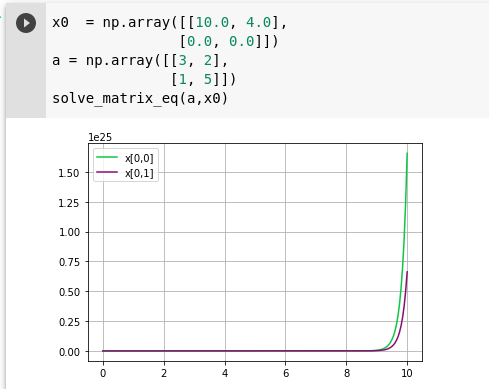
\includegraphics[width=9cm]{fig12}}
	\caption{جواب تخمینی معادله 
		\ref{eq:sysdiff}	
	}
	\label{fig:fig12}
\end{figure}